\documentclass{beamer}
\usepackage{siunitx,booktabs,xcolor,xspace,multirow,graphicx,lipsum}
\usepackage[spanish,mexico,es-noindentfirst]{babel}
\usepackage[utf8]{inputenc}
\usepackage{tikz}
\usetikzlibrary{shapes,arrows.meta,positioning,calc,fit,backgrounds,shadows,decorations.pathreplacing}
\usepackage{subcaption}
\usepackage[charter]{mathdesign}
\usetheme{Madrid}
\usepackage{tcolorbox}
\usepackage{hyperref}

\usefonttheme{serif}


\setbeamertemplate{frametitle}{
  \begin{beamercolorbox}[wd=\paperwidth,ht=1cm, sep=0.25cm]{frametitle}
    \begin{tikzpicture}[remember picture,overlay]
      \node[anchor=north east] at (current page.north east) {
\includegraphics[height=0.75cm]{figuras/inetSys-fundo-azul-logo.png}};
    \end{tikzpicture}
    \usebeamerfont{frametitle}\bfseries\insertframetitle
  \end{beamercolorbox}
}

\setbeamertemplate{caption}[numbered]
\setbeamercolor{frametitle}{bg=beamer_color,fg=white}
\setbeamercolor{author in head/foot}{bg=beamer_color,fg=white}
\setbeamercolor{title in head/foot}{bg=beamer_color,fg=white}
\setbeamercolor{date in head/foot}{bg=beamer_color,fg=white}
\setbeamercolor{titlelike}{parent=structure,bg=beamer_color,fg=white}
\setbeamertemplate{section in toc}[sections numbered]
\setbeamertemplate{subsection in toc}[subsections numbered]
\setbeamerfont{section in toc}{series=\bfseries}
\setbeamercolor{section in toc}{fg=black}
\setbeamercolor{caption name}{fg=blue}
\setbeamerfont{caption name}{series=\bfseries}
\setbeamerfont{caption}{size=\small}
\setbeamercolor{bibliography entry author}{fg=black}
\setbeamercolor{bibliography entry title}{fg=black} 
\setbeamertemplate{section in toc}{\inserttocsectionnumber.~\inserttocsection\par}
\setbeamertemplate{subsection in toc}{\hspace{1.5em}\inserttocsectionnumber.\inserttocsubsectionnumber~\inserttocsubsection\par}



\title[\textbf{}]{\textbf{SAC-FTOPSIS: Um Modelo de Decisão para o Descarregamento de Tarefas em Redes Veiculares}}
\author[\textbf{Antônio Sérgio de Sousa Vieira}]{\textbf{Antônio Sérgio de Sousa Vieira \break sergio.vieira@ifce.edu.br}}
\date{}

\renewcommand{\maketitle}{
\begin{center}
    
\includegraphics[height=0.8cm]{figuras/ifce.pdf}\hspace{0.5cm}
    
\includegraphics[height=0.8cm]{figuras/uece_inetsys_desc_logo.png}
    \\[0.1cm]
    \textbf{\scriptsize DOUTORADO EM CIÊNCIA DA COMPUTAÇÃO}
\end{center}

\vspace{-1.8\baselineskip}
\titlepage
\vspace{-3.2\baselineskip}

\begin{center}
    \tiny
    \begin{tabular}{rl}
        \textbf{Orientador:} & Dr. Joaquim Celestino Júnior (UECE) \\
        \textbf{Coorientador:} & Prof. Dr. Alisson Barbosa de Souza (UFC) \\
    \end{tabular}

    \vspace{0.1cm}
    \textbf{Banca Examinadora:} \\
    \begin{tabular}{c}
        Prof. Dr. Luís Manuel De Jesus Sousa Correia (ULisboa) \\
        Prof. Dr. Gustavo Augusto Lima de Campos (UECE) \\
        Prof. Dr. Eduardo de Olivindo Cavalcante (IFCE)
    \end{tabular}
    
    \vspace{0.2cm}
    \textbf{29 de maio de 2026}
\end{center}
}

% \AtBeginSection[ ]
% {
% \begin{frame}{Contenido de la presentación}
% \tableofcontents[currentsection,subsectionstyle = shaded]
% \end{frame}
% }

% \AtBeginSubsection[ ]
% {
% \begin{frame}{Contenido de la presentación}
% \tableofcontents[currentsection,currentsubsection]
% \end{frame}
% }

% Definir color verde
% \definecolor{beamer_color}{RGB}{64, 145, 63}
% \definecolor{backframe_color}{RGB}{228, 242, 232}

% Definir color morado
\definecolor{beamer_color}{RGB}{0,0,153} 
\definecolor{backframe_color}{RGB}{235, 196, 245}


\begin{document}

\begin{frame}
    \maketitle
\end{frame}

\begin{frame}{Agenda}
    \tableofcontents
\end{frame}

% \section{O Desafio}

% \begin{frame}{O Desafio}
%     \vspace{0.8cm}
%     \centering
%     \LARGE \bfseries
%     Como decidir o descarregamento se a\\[0.4cm]
%     \tikz[baseline=(box.base)] \node[fill=blue!15, rounded corners=2pt, inner sep=5pt] (box) {topologia da rede}; muda\\[0.4cm]
%     na mesma hora?
% \end{frame}

%%\section{Agenda}

\section{Introdução}

%%################## Slide PERFIS DE APLICAÇÃO ##################
\begin{frame}{Perfis de Aplicação e Desafios de ITS}
    \begin{columns}[T]
        \begin{column}{0.48\textwidth}
            \begin{tcolorbox}[colback=blue!5, colframe=beamer_color, title=Cenário V2X (Cruzamento), fonttitle=\bfseries\footnotesize, arc=0pt, outer arc=0pt, leftrule=3pt, rightrule=0.3pt, toprule=0.1pt, bottomrule=0.3pt]
                \scriptsize 
                \textbf{Elementos (Fig.)}: Veículo cliente ($v_0$), vizinhos cooperativos ($v_1, v_2$) e infraestrutura (RSU).\\
                \textbf{Conectividade}: Links ativos V2I (via 5G) e V2V (Sidelink).
            \end{tcolorbox}
            
            \vspace{-0.45cm}
            
            \begin{tcolorbox}[colback=orange!5, colframe=orange!80!black, title=Perfis de Tarefa Gerados, fonttitle=\bfseries\footnotesize, arc=0pt, outer arc=0pt, leftrule=3pt, rightrule=0.3pt, toprule=0.3pt, bottomrule=0.3pt]
                \scriptsize 
                \textbf{Segurança (Vermelho)}: Alertas críticos com prazo rígido ($\le 100$ms).\\
                \textbf{Visão/Fusão (Laranja)}: Percepção cooperativa de alta complexidade ($>250$k ciclos/byte).
            \end{tcolorbox}
            
            \vspace{-0.45cm}
            
            \begin{tcolorbox}[colback=red!5, colframe=red!70!black, title=Gargalo Local e Decisão, fonttitle=\bfseries\footnotesize, arc=0pt, outer arc=0pt, leftrule=3pt, rightrule=0.3pt, toprule=0.3pt, bottomrule=0.3pt]
                \scriptsize 
                \textbf{Gargalo Local}: Limites térmicos/bateria no OBUI de $v_0$ (alerta \textbf{!} em vermelho na Fig.).\\
                \textbf{Problema}: Escolher o destino (Local, RSU ou Vizinhos) que maximiza o cumprimento de prazos.
            \end{tcolorbox}
        \end{column}
        
        \begin{column}{0.52\textwidth}
            \centering
            \vspace{0.1cm}
            \begin{tikzpicture}[
                scale=0.45,
                transform shape,
                every node/.style={inner sep=2pt},
                vehicle/.style={draw=orange!80!black, fill=orange!10, minimum width=1.4cm, minimum height=0.65cm, rounded corners=2pt, font=\bfseries\tiny, align=center, thick},
                client/.style={draw=beamer_color, fill=beamer_color!15, minimum width=1.4cm, minimum height=0.65cm, rounded corners=2pt, font=\bfseries\tiny, align=center, thick},
                rsu/.style={draw=purple, fill=purple!5, minimum width=1.3cm, minimum height=1.3cm, rounded corners=3pt, font=\bfseries\tiny, align=center, thick},
                task_s/.style={draw=red, fill=red!5, rounded corners=2pt, font=\fontsize{5}{6}\selectfont, align=center},
                task_c/.style={draw=orange, fill=orange!5, rounded corners=2pt, font=\fontsize{5}{6}\selectfont, align=center},
                link_v2i/.style={purple, dashed, ultra thick, <->},
                link_v2v/.style={orange!80!black, dotted, ultra thick, <->}
            ]
                % Draw Roads (gray intersection)
                \fill[gray!20] (-5,-2) rectangle (5,2);
                \fill[gray!20] (-2,-5) rectangle (2,5);
                
                % Road borders (dark gray)
                \draw[gray!50, thick] (-5,2) -- (-2,2) -- (-2,5);
                \draw[gray!50, thick] (5,2) -- (2,2) -- (2,5);
                \draw[gray!50, thick] (-5,-2) -- (-2,-2) -- (-2,-5);
                \draw[gray!50, thick] (5,-2) -- (2,-2) -- (2,-5);
                
                % Lane dividers (white dashed)
                \draw[white, dashed, thick] (-5,0) -- (-2,0);
                \draw[white, dashed, thick] (2,0) -- (5,0);
                \draw[white, dashed, thick] (0,-5) -- (0,-2);
                \draw[white, dashed, thick] (0,2) -- (0,5);
                
                % Pedestrian crossings (zebra lines)
                \foreach \x in {-1.6,-1.2,-0.8,-0.4,0,0.4,0.8,1.2,1.6} {
                    \draw[white, line width=1.5pt] (\x, 2.1) -- (\x, 2.4);
                    \draw[white, line width=1.5pt] (\x, -2.1) -- (\x, -2.4);
                    \draw[white, line width=1.5pt] (2.1, \x) -- (2.4, \x);
                    \draw[white, line width=1.5pt] (-2.1, \x) -- (-2.4, \x);
                }
                
                % Elements placing
                % Client Vehicle v0
                \node[client] (v0) at (-0.8, -1.0) {$v_0$ \\ \textbf{Cliente}};
                
                % Neighboring Vehicles (v1 and v2)
                \node[vehicle] (v1) at (0.8, 3.2) {$v_1$ \\ \textbf{Vizinho}};
                \node[vehicle] (v2) at (-3.5, 0.8) {$v_2$ \\ \textbf{Vizinho}};
                
                % RSU Tower (MEC Server) at Top-Right
                \node[rsu] (rsu) at (3.5, 3.5) {RSU / MEC \\ \textbf{Server}};
                % Signal waves at RSU
                \draw[purple, thin] ([yshift=1mm]rsu.north) arc (90:45:5mm);
                \draw[purple, thin] ([yshift=1mm]rsu.north) arc (90:135:5mm);
                \draw[purple, thin] ([yshift=3mm]rsu.north) arc (90:45:8mm);
                \draw[purple, thin] ([yshift=3mm]rsu.north) arc (90:135:8mm);
                
                % Communication links
                % V2I from v0 to RSU
                \draw[link_v2i] (v0) to[bend right=15] node[midway, right=1pt, font=\fontsize{5}{6}\selectfont, text=purple] {V2I (5G)} (rsu);
                
                % V2V from v0 to v1, v2
                \draw[link_v2v] (v0) -- node[midway, right=1pt, font=\fontsize{5}{6}\selectfont, text=orange!80!black] {V2V Sidelink} (v1);
                \draw[link_v2v] (v0) -- node[midway, below=1pt, font=\fontsize{5}{6}\selectfont, text=orange!80!black] {V2V Sidelink} (v2);
                
                % Task bubble generating from v0
                \node[task_s] (t_safety) at (-3.6, -3.2) {\textbf{Alerta (Segurança)} \\ $\le 100$ms Deadline};
                \node[task_c] (t_compute) at (0.0, -3.5) {\textbf{Fusão (Visão)} \\ $>250$k ciclos/B};
                
                % Arrows from tasks to v0
                \draw[-{Stealth[scale=0.8]}, thick, red] (t_safety) to[bend left=10] (v0);
                \draw[-{Stealth[scale=0.8]}, thick, orange] (t_compute) to[bend right=10] (v0);
                
                % Local bottleneck indicator at v0
                \node[draw=red, circle, fill=red!20, inner sep=1pt, font=\tiny\bfseries] (warn) at (-1.8, -1.0) {!};
                \node[text=red, font=\fontsize{5}{6}\selectfont, anchor=east, align=center] at (warn.west) {OBUI \\ Sobregregado};
                \draw[red, thin] (warn) -- (v0);
            \end{tikzpicture}
            
            \vspace{0.1cm}
            \begin{beamercolorbox}[wd=\textwidth, sep=4pt, center, rounded=true]{block body}
                \scriptsize \textit{"A viabilização do ITS de próxima geração depende da superação das limitações computacionais locais."}
            \end{beamercolorbox}
        \end{column}
    \end{columns}
\end{frame}

%%################## Slide INTRODUÇÃO ###################
\begin{frame}{Computação Cooperativa e Offloading}
    \begin{columns}[T]
        \begin{column}{0.48\textwidth}
            \begin{tcolorbox}[colback=blue!5, colframe=beamer_color, title=Heterogeneidade e Cooperação, fonttitle=\bfseries\footnotesize, arc=0pt, outer arc=0pt, leftrule=3pt, rightrule=0.3pt, toprule=0.3pt, bottomrule=0.3pt]
                \scriptsize 
                \textbf{Capacidades}: OBUIs possuem hardware e níveis de bateria distintos.\\
                \textbf{Compartilhamento}: Veículos vizinhos podem ceder recursos ociosos.
            \end{tcolorbox}
            
            \vspace{-0.1cm}
            
            \begin{tcolorbox}[colback=orange!5, colframe=orange!80!black, title=A Estratégia de Offloading, fonttitle=\bfseries\footnotesize, arc=0pt, outer arc=0pt, leftrule=3pt, rightrule=0.3pt, toprule=0.3pt, bottomrule=0.3pt]
                \scriptsize Essencial para superar gargalos locais de processamento em tarefas complexas e sensíveis ao atraso.
            \end{tcolorbox}
            
            \vspace{-0.1cm}
            
            \begin{tcolorbox}[colback=red!5, colframe=red!70!black, title=O Desafio Crítico, fonttitle=\bfseries\footnotesize, arc=0pt, outer arc=0pt, leftrule=3pt, rightrule=0.3pt, toprule=0.3pt, bottomrule=0.3pt]
                \scriptsize \textbf{Decisão}: Como e onde descarregar em topologias altamente dinâmicas e imprevisíveis?
            \end{tcolorbox}
        \end{column}
        
        \begin{column}{0.52\textwidth}
            \centering
            \vspace{0.2cm}
            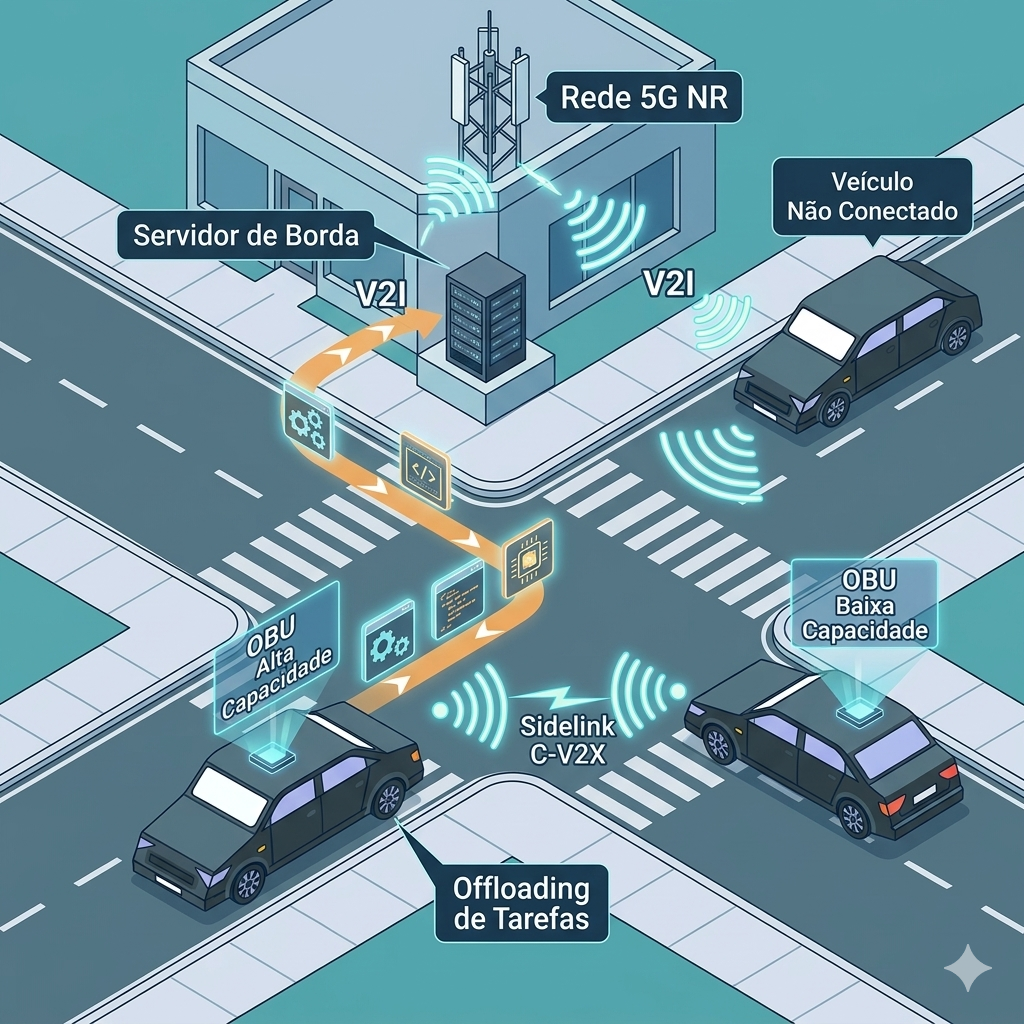
\includegraphics[width=\textwidth]{figuras/cenario.png}
            
            \vspace{0.1cm}
            \begin{beamercolorbox}[wd=\textwidth, sep=4pt, center, rounded=true]{block body}
                \scriptsize \textit{"O offloading não é apenas uma opção, mas uma necessidade em cenários de alta demanda."}
            \end{beamercolorbox}
        \end{column}
    \end{columns}
\end{frame}

\begin{frame}{Limitações das Abordagens Tradicionais}
    \begin{block}{Heurísticas e MCDM}
        \begin{itemize}
            \item Simplicidade computacional.
            \item \textbf{Falha}: Avaliam apenas o estado instantâneo (sem visão de futuro).
        \end{itemize}
    \end{block}
    
    \begin{block}{Meta-heurísticas (Algoritmos Genéticos, PSO, etc.)}
        \begin{itemize}
            \item Busca global sólida em cenários estáticos.
            \item \textbf{Falha}: Convergência lenta (incompatível com prazos de milissegundos).
            \item \textbf{Inflexibilidade}: Precisam ser reiniciadas a cada mudança na topologia.
        \end{itemize}
    \end{block}
\end{frame}

\begin{frame}{O Desafio da Generalização}
    \begin{itemize}
        \item \textbf{Modelos Simplificados}: Cenários com número fixo de veículos não capturam a realidade.
        \item \textbf{Degradação de Desempenho}: Mudanças súbitas na densidade invalidam políticas rígidas.
        \item \textbf{Necessidade de Robustez}: Representações de estado que garantam a generalização sem necessidade de retreinamento constante.
    \end{itemize}
\end{frame}

\begin{frame}{Aprendizado por Reforço Profundo (DRL)}
    \begin{itemize}
        \item \textbf{Solução Natural}: Aprende políticas de controle mapeando observações em ações de longo prazo.
        \item \textbf{Exploração Temporal}: Identifica padrões em tráfego, filas e mobilidade.
        \item \alert{Fraqueza Estrutural}: Dependência de camadas de entrada com tamanho fixo.
        \item \alert{Gargalo}: Exige retreinamento sempre que a quantidade de nós candidatos muda.
    \end{itemize}
\end{frame}


% \section{Imagens}
% %%################ Imagens #############
% \begin{frame}{Imagens}
%     Carregar imagem na pasta \texttt{figuras}. 

%    A Figura \ref{fig:red_ramificada} mostra um exemplo de como inserir a imagem e referência.

%     \begin{figure}[htbp]
%         \centering
%         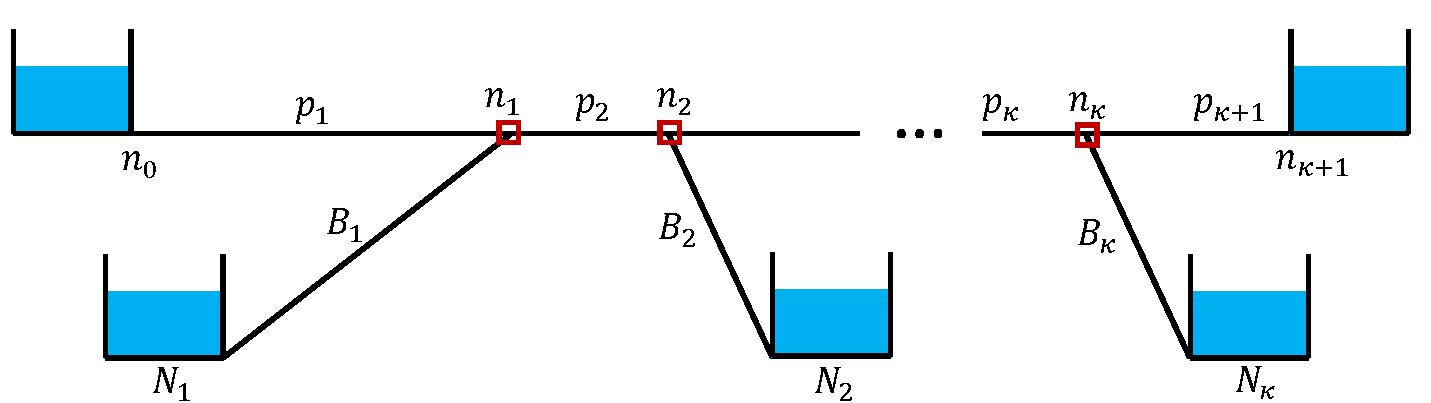
\includegraphics[width = \textwidth]{figuras/BranchedScheme.pdf} % Usar a sua imagem
%         \caption{Rede com $k$ ramificações.} % Referência
%         \label{fig:red_ramificada} % Label
%     \end{figure}
% \end{frame}

% %%################ Imagens Slide 2 #############
% \begin{frame}{Imagens Slide 2}

%     A Figura \ref{fig:comparacion_redes} mostra como inserir figuras lado a lado.

%     \begin{figure}[htbp]
%     \centering
%     \begin{subfigure}[b]{0.48\textwidth}
%         \centering
%         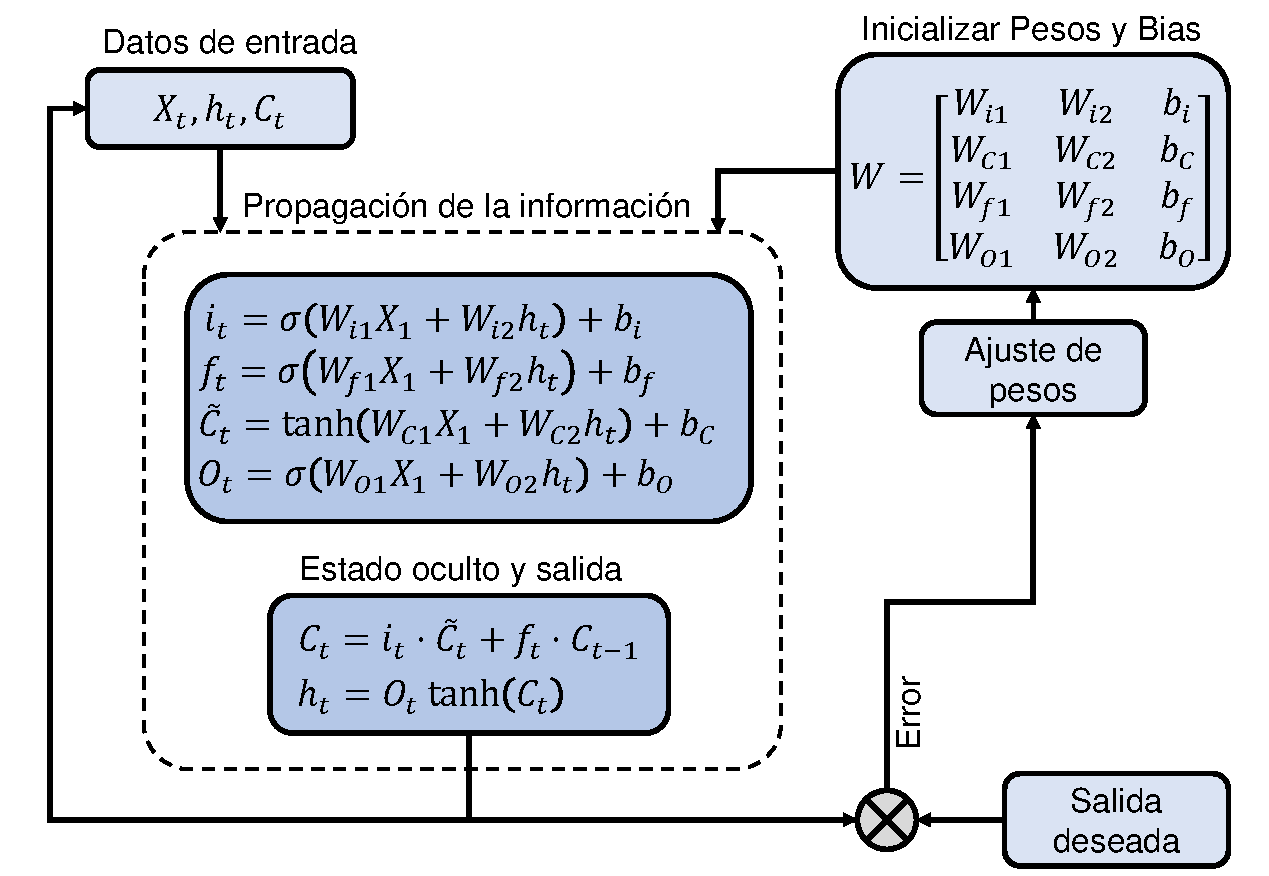
\includegraphics[width=\textwidth]{figuras/LSTM.pdf}
%         \caption{Red LSTM}
%         \label{fig:figura1a}
%     \end{subfigure}
%     \hfill
%     \begin{subfigure}[b]{0.48\textwidth}
%         \centering
%         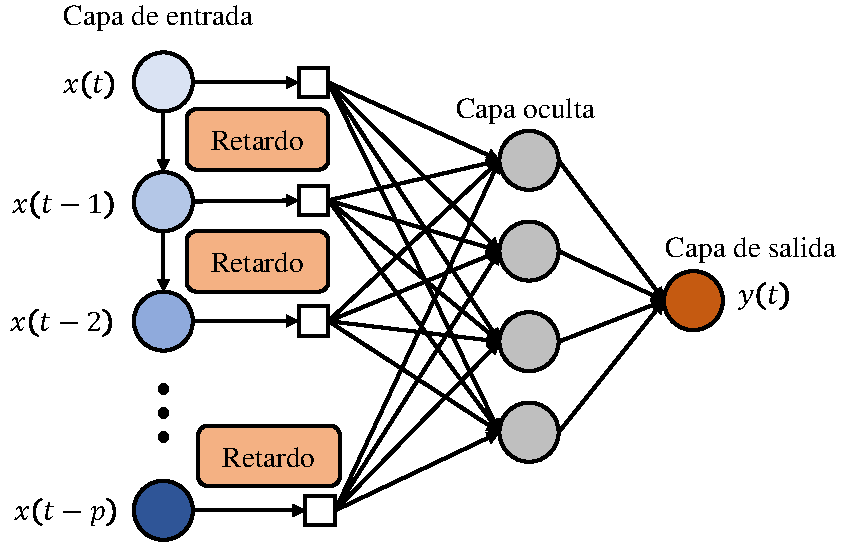
\includegraphics[width=\textwidth]{figuras/TDNN.pdf}
%         \caption{Red TDNN}
%         \label{fig:figura1b}
%     \end{subfigure}
%     \caption[Comparação entre redes neurais]{Comparação entre redes neurais}
%     \label{fig:comparacion_redes}
% \end{figure}
    
% \end{frame}


% \section{Equações}
% %%################ Equações #############
% \begin{frame}{Equações}

%     Exemplo de equação numerada:
%     \begin{equation}
%         \frac{\partial Q\left(z_k,t\right)}{\partial t}+gA_k\frac{\partial H\left(z_k,t\right)}{\partial z_k}+\mu_kQ\left(z_k,t\right)\left|Q\left(z_k,t\right)\right|+g\sin{a_k}=0,
%         \label{eq:momentum}
%     \end{equation}
%     Uma equação numerada se referencia no texto usando seu \textit{label}: A Equação \eqref{eq:momentum} é conhecida como a Equação de Momentum.
    
%     Exemplo de uma equação sem numeração:
%     $$\frac{\partial H\left(z_k,t\right)}{\partial t}+\frac{b_k^2}{gA_k}\frac{\partial Q\left(z_k,t\right)}{\partial z_k}=0.$$

%     Exemplo da equação no texto: $\mu_k=\frac{fQ_k}{2D_kA_k}$  
% \end{frame}


% \section{Tabelas}
% %%################ Tabelas #############
% \begin{frame}{Tabelas}
%     A Tabela \ref{tab:ModelosPerdida} mostra uma tabela de uma coluna. 
    
%     \begin{table}[htbp]
%         \centering
%          \caption{Fórmulas para o cálculo de perdas de carga em tubulações.\break}
%          \vspace{-\baselineskip}
%         \label{tab:ModelosPerdida}
%         \small
%         \begin{tabular}{ccc}
%             \toprule
%             \textbf{Perda} & \textbf{Coeficiente} $C$ & \textbf{Exponente} $\sigma$ \\
%             \midrule
%             Hazen-Williams & $4.727 \mathscr{H}^{-1.852}D^{-4.871}L$ & 1.852 \\
%             Darcy-Weisbach & $0.0252f(\varepsilon, D, Q)D^{-5}L$ & 2 \\
%             Chezy-Manning & $4.66n^2D^{-5.33}L$ & 2 \\
%             \bottomrule
%         \end{tabular}
%     \end{table}
    
% \end{frame}


% %%################ Tabelas Slide 2#############
% \begin{frame}{Tabelas Slide 2}

%     A Tabela \ref{Tab:Accesorios} mostra um exemplo de duas colunas.
    
%     \begin{table}[htbp]
%         \centering
%         \caption{Acessórios}
%         \vspace{-\baselineskip}
%         \label{Tab:Accesorios}
%         \null\hfill
%         \scriptsize
%         \begin{tabular}{cl}
%         % \multicolumn{2}{c}{a) Tuberías 1-8}\\[2pt]
%         \toprule
%         \textbf{Coluna 01} & \textbf{Coluna 02} \\
%         \midrule
%         $\text{N}_{1}-\text{N}_{2}$ & 2 Codos 90°\\
%         $\text{N}_{2}-\text{N}_{3}$ & 4 Codos 90° \\ 
        
%         $\text{N}_{4}-\text{N}_{5}$ & 2 Codos 90° \\ 
%         $\text{N}_{5}-\text{N}_{6}$ & 4 Codos 90° \\ 
        
%         $\text{N}_{7}-\text{N}_{8}$ & 2 Codos 90° \\
%         $\text{N}_{8}-\text{N}_{9}$ & 4 Codos 90° \\ 
%         \bottomrule
%         \end{tabular}
%         \hfill\hfill
%         \begin{tabular}{cl}
%         % \multicolumn{2}{c}{b) Tuberías 9-16}\\[2pt]
%         \toprule
%         \textbf{Coluna 01} & \textbf{Coluna 02} \\
%         \midrule
%         $\text{N}_{4}-\text{N}_{10}$ & 1 Codo 90°, 1 Valvula, 1 T \\ 
        
%         $\text{N}_{11}-\text{N}_{12}$ & 4 Codos 90° \\ 
%         $\text{N}_{12}-\text{N}_{13}$ & 2 Codos 90° \\ 
%         $\text{N}_{6}-\text{N}_{14}$ & 1 Codo 90°, 1 Valvula, 1 T \\ 
        
%         $\text{N}_{15}-\text{N}_{16}$ & 2 Codos 90° \\ 
%         $\text{N}_{16}-\text{N}_{17}$ & 4 Codos 90° \\ 
%         \bottomrule
%         \end{tabular}
%         \hfill\null
%     \end{table}
    
% \end{frame}


\section{Referências}
%%################ Referências #############
\begin{frame}{Referências}
    Adicione as referêcnias no documento  \texttt{biblio.bib} no formato \texttt{BibTex}.

    Exemplo de uma referência \cite{zhang2017digital}.
    Exemplo de duas ou mais referências em uma citação, separado com vírgulas \cite{praks2018advanced,santos2018online}.
    As referências são adiconadas automaticamente na Bibliografia.
\end{frame}

\begin{frame}[allowframebreaks]{Bibliografia}
\bibliographystyle{ieeetr}
\bibliography{biblio}
\end{frame}


\begin{frame}
    \maketitle
\end{frame}


\end{document}